\documentclass{article} % For LaTeX2e
\usepackage{nips2015,times}
\usepackage{hyperref}
\usepackage{url}
\usepackage{graphicx}
\graphicspath{ {../assets/} }
\usepackage{biblatex}
\addbibresource{refs.bib}


\usepackage{float}
\usepackage[inline]{enumitem}
\usepackage{booktabs}
\usepackage{multirow}
\usepackage[center]{caption}
\usepackage{subcaption}

\title{CSE 546 Assignment 1}


\author{
   Mohammed Nasheed Yasin \\
   Department of Linguistics\\
   University at Buffalo, SUNY\\
   Buffalo, NY 14260 \\
   \texttt{m44@buffalo.edu}
}

% The \author macro works with any number of authors. There are two commands
% used to separate the names and addresses of multiple authors: \And and \AND.
%
% Using \And between authors leaves it to \LaTeX{} to determine where to break
% the lines. Using \AND forces a linebreak at that point. So, if \LaTeX{}
% puts 3 of 4 authors names on the first line, and the last on the second
% line, try using \AND instead of \And before the third author name.

\newcommand{\fix}{\marginpar{FIX}}
\newcommand{\new}{\marginpar{NEW}}

\nipsfinalcopy

\begin{document}


\maketitle

\begin{abstract}
    This report explains our\footnote{Although this work has been written in first person plural (we/ours)
    this is the work of only the listed author. Such a convention has been adopted to keep
    in line with paper writing tradition.} experiments with environments in RL.
    It focuses on the differences between stochastic and deterministic environments,
    and introduces commonly used rendering methodologies. We also go on to solve these
    environments with popular RL tabular methods: Q and Double Q Learning.
\end{abstract}

\section{The Environments}
\label{sec:definition}

There are certain features that are common to both the stocastic and deterministic environments.

\subsection*{Environmental Elements}
\begin{figure}[h]
    \begin{center}
        
\includegraphics[width=\textwidth]{elements.png}
    \end{center}
    \caption{Environmental elements (from left to right; top to bottom) Agent, Goal,
        Negative Reward, Reward}
    \label{fig:elements}
\end{figure}

The enivironment is a \verb|6x6| grid defined according to the Gym \cite{1606.01540} API.
With \verb|36| possible positions that the agent can
occupy. The goal is to reach the oasis (shown in Figure \ref{fig:elements}) \textbf{after
consuming all} the juice (positive reward) within a (configurable) maximum number of time
steps. If the agent lands on a juice tile it is awarded +0.99 and the cactus (negative
reward) leads to a -1.0 reward. Once all the juice is consumed, the agent must proceed to the
oasis to earn a reward of +1.0
The states in this enviroment are a \textbf{combination} of the agent's position and the
currently available rewards (positive, negative and goal) on the grid. The Formula
\ref{eqn:num-states} gives us the number of possible states for the agent.

\begin{equation}
    num_{states}=num_{pos} \sum_{k=0}^{c_{reward}} {c_{reward}\choose k}
    \label{eqn:num-states}
\end{equation}

Here $num_{pos}$ refers to the number of grid squares, \verb|36| in our case. $c_{reward}$
refers to the number of positive rewards + the number of negative rewards + 1 (for the goal
state). We have \verb|6| negative rewards, \verb|3| positive rewards and one goal. Hence, 
the $num_{states}$ for us is \verb|36864|.

In each position our agent can take 4 potential actions:
\begin{enumerate*}
    \item Left
    \item Right
    \item Up
    \item Down.
\end{enumerate*}
Resetting the environment will not change the location or distribution of the rewards and
goal state. It only alters the initial state of the agent.

\begin{figure}[h]
    \begin{center}
        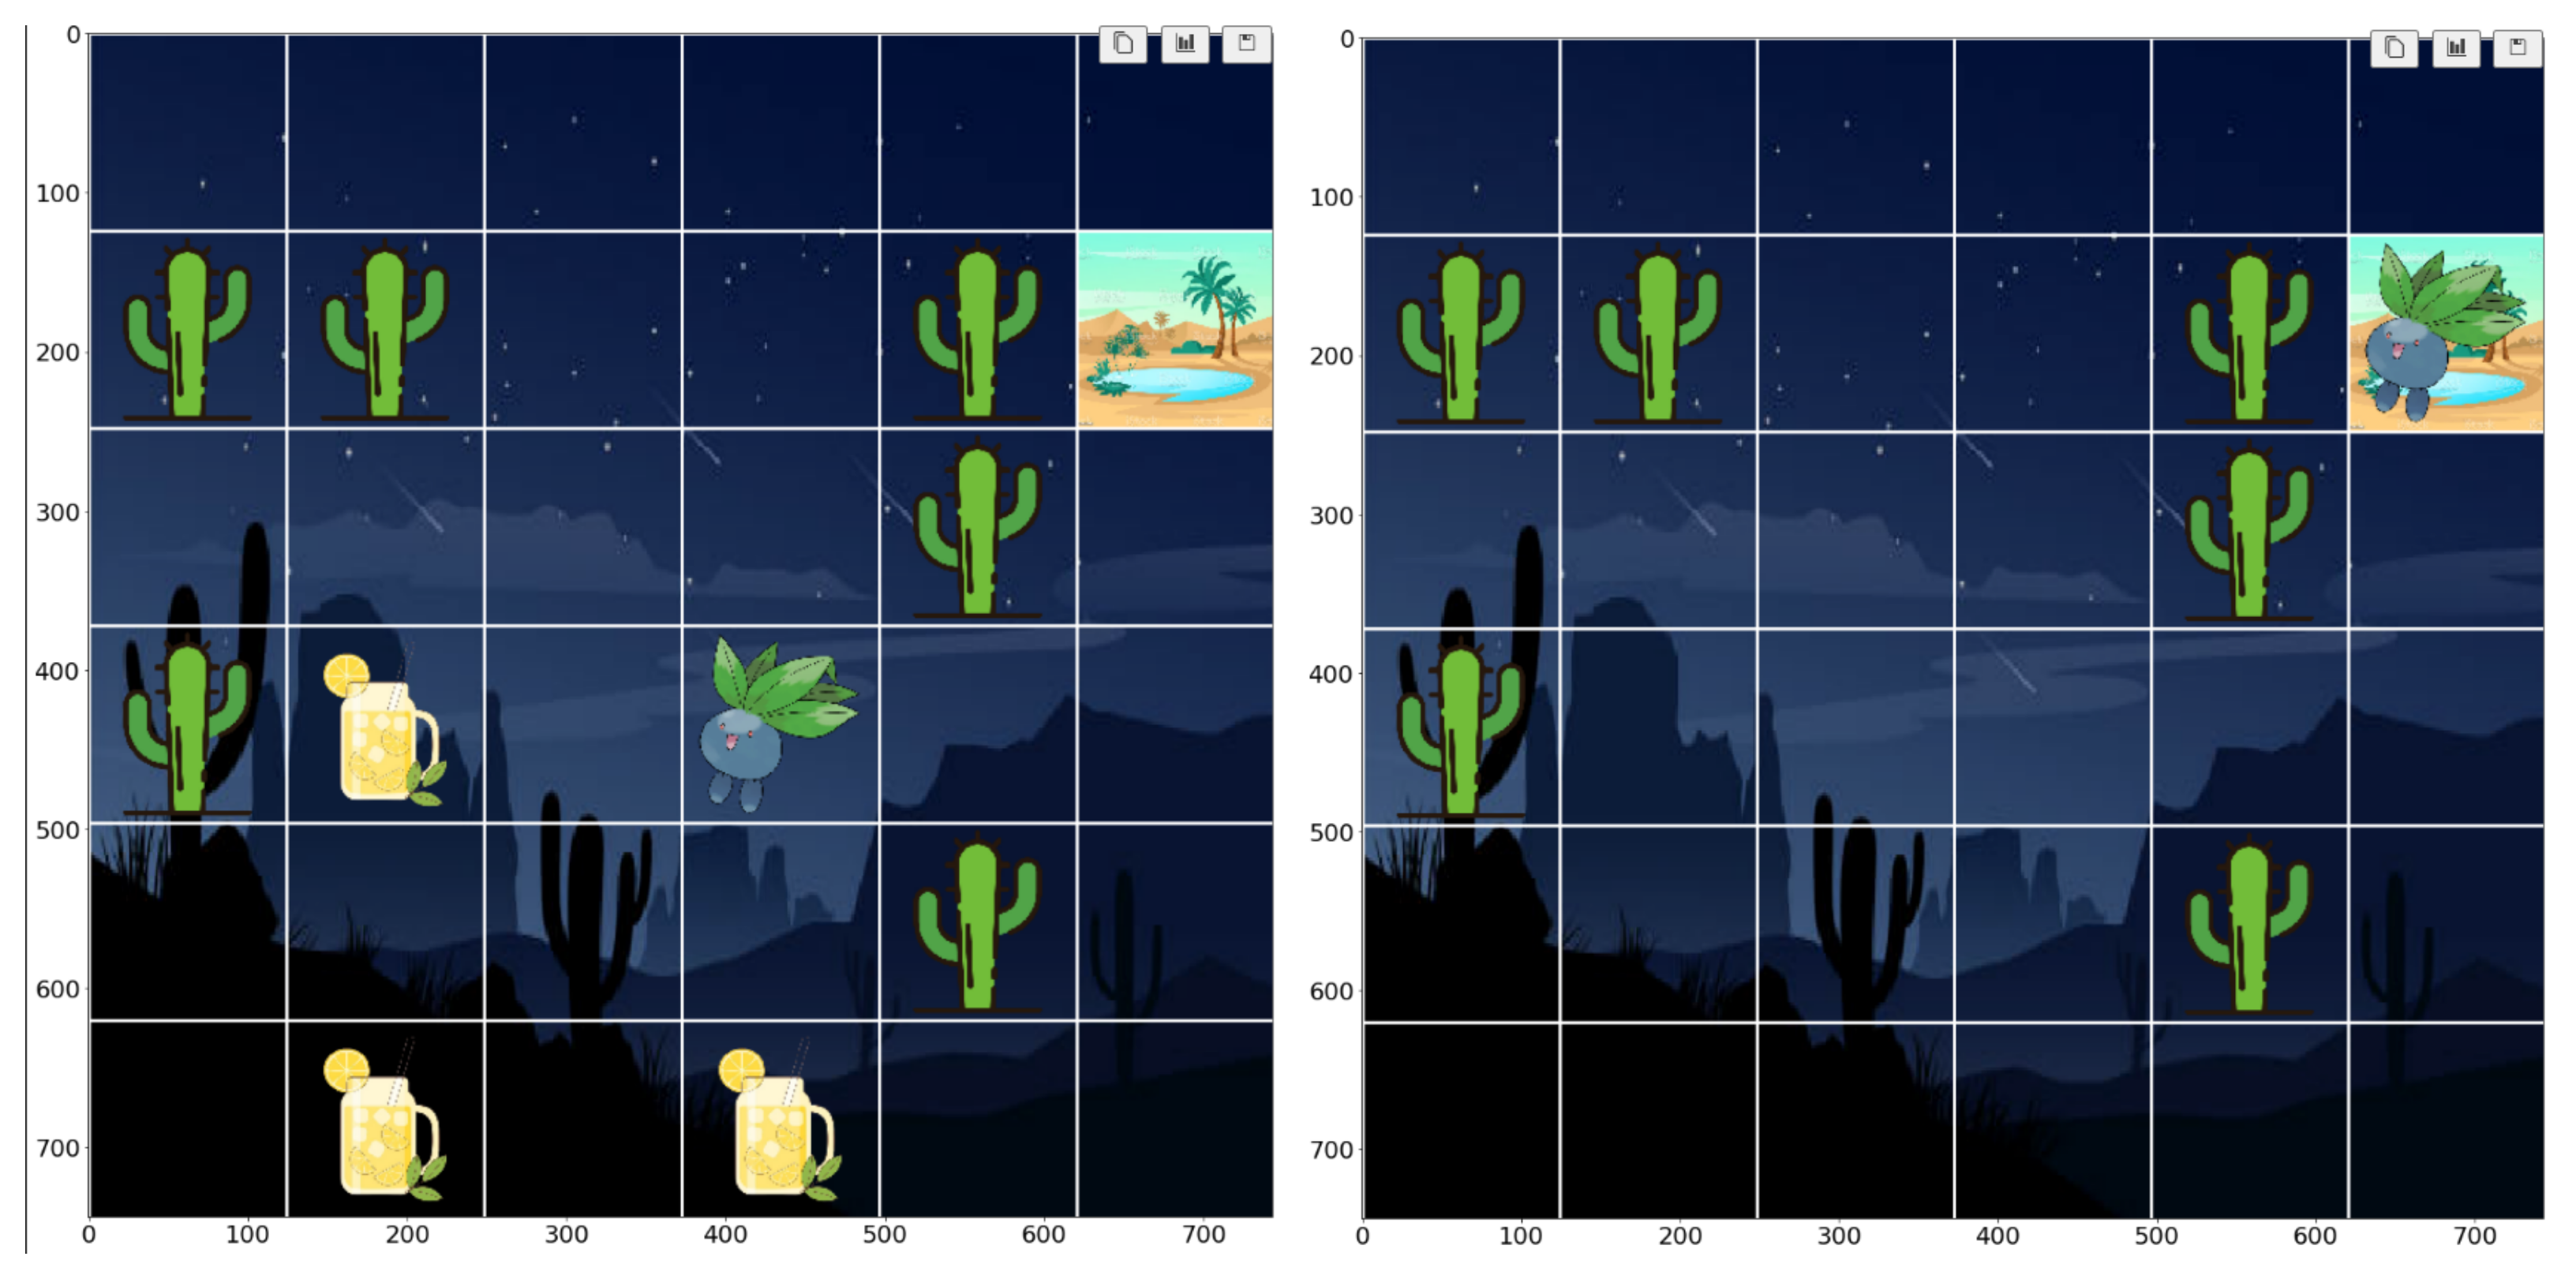
\includegraphics[scale=0.50]{vis.png}
    \end{center}
    \caption{Environment visualizations}
\end{figure}


\subsection{Stocasticity}

\label{sec:sto}
An enviroment is called stocastic when the result of an action (i.e. its success or its 
reward) is not guaranteed. Formally, given the same state $s_0$ and action $a$ the next state
$s_1$ and reward $r$ will be probability distributions.

In our \verb|GridEnviroment| the stocasticity can be described as follows:
\begin{itemize}
    \item For every action there is a $2/3^{rd}$ chance that the action is performed as
        expected (\verb|as-is|), a $2/9^{th}$ chance that it is the \verb|double| of what 
        is expected and a $1/9^{th}$ chance of it being a \verb|mirror| action.
    \item A bonus is distributed in a reciprocal proportions. i.e. \verb|0.1x| the
        \verb|max_reward| for coming through the \verb|as-is| action, \verb|0.2x| \verb|max_reward|
        for coming via the \verb|double| action and \verb|0.3x| \verb|max_reward| for the
        \verb|mirror| action.
    \item For instance on a 6x6 grid where the reward on each square is 1 (for simplicity):
    \newline
    If $s_0$ \verb|=(2,3)| and $a$ \verb|= RIGHT|:
        \begin{itemize}
            \item $2/3^{rd}$ chance $s_1$ \verb|=(2,4)| and $r$ \verb|=1+0.1|
            \item $2/9^{th}$ chance $s_1$ \verb|=(2,5)| and $r$ \verb|=1+0.2|
            \item $1/9^{th}$ chance $s_1$ \verb|=(3,2)| and $r$ \verb|=1+0.3|
        \end{itemize}
\end{itemize}

\subsection{Safety in AI}
\label{sec:safety}
The following are properties of the environment that ensure valid behavior from the agent:

\begin{enumerate}
    \item We ensure that the agent consumes \textit{all} the \verb|pos_reward| and reaches
        the \verb|goal_state| in the fewest number of steps by imposing a penalty of \verb|0.1x|
        the \verb|max_reward| for every move made.
    \item The reward on all squares is consumed once the agent lands in that state, preventing 
    the agent from settling down in a \textit{high-reward} neighborhood.
    \item The result of any action (left, right, top, down) are clipped to the min and max
        values of 0 and \verb|GridSize| (6 in our case) respectively, ensuring that the
        agent never leaves the environment.
    \item If the agent makes a move but remains in the same spot, we impose the \textit{maximum negative
        reward} (-1.0 in our case). This allows the agent to disincentivize making fruitless
        moves.
    \item We also prevent a \textit{goal rush} (before the agent consumes all the positive
        rewards) by making the goal square unreachable when there are positive reward squares
        left. If the agent takes an action to move into a goal square before collecing all the
        \textit{positive rewards}, they will be kept on the same square, incurring an additional
        penalty (-1.0 in our case) as detailed in the previous point.
    \item The stocasticity of the starting point and limited time steps will nudge the agent
        to build strategies that accumulate the maximal reward in the shortest time.
\end{enumerate}

\section{Tabular Methods}
We applied the Q Learning and Double Q learning tabular methods to solve the environment
defined in section \ref{sec:definition}. Both these techniques fall under the Temporal 
Difference (TD) \textit{model-free} category and we estimate the Q value of each state action pair
by considering as target the sum of the reward and the Q value of the next state action pair.
Since we only consider the immediately following state's Q value and reward, we call it a TD(0)
approach.

\begin{equation}
    Q(S,A)_Q = Q(S,A)_Q + \alpha[R+\gamma max_a Q(S', a)_Q-Q(S,A)_Q]
    \label{eqn:q-update}
\end{equation}

Equation \ref{eqn:q-update} is the update function for Q Learning where the $\alpha$ refers
to the \textit{learning rate} and the $\gamma$ represents the \textit{discount factor}. The
target value of each state-action pair is represented by $R+\gamma max_a Q(S', a)_Q$. Here
$R$ is the reward recieved by taking action $A$ at state $S$.

Double Q Learning is an extention to Vanilla Q Learning which uses two Q tables instead of one.
It targets the over-estimation issue that afflicts Q Learning as it is unlikely that both the
Q tables over-estimate the same set of state-action pairs. Such a set-up therefore allows
faster convergence of the learning algorithm. Essentially, at each time step we choose the
action according to a \textit{mean Q table} (in our case), collect the reward and \textit{randomly}
choose to update one of the two Q tables.

For instance if we choose to update table A. Then we choose the greedy action for the state
$S'$ according to table A. But the value for this action is taken from table B. Equation
\ref{eqn:dbq-update} formally states the update mechanism. The symbols mean the same as they
did in Q learning update (Equation \ref{eqn:q-update}).


\begin{equation}
    Q(S,A)_{DbQ}^A = Q(S,A)_{DbQ}^A + \alpha[R+\gamma Q(S', argmax_a Q(S', a)_{DbQ}^A)_{DbQ}^B-Q(S,A)_{DbQ}^A]
    \label{eqn:dbq-update}
\end{equation}

Q Learning and Double Q Learning are defined as off-policy methods since the target is
estimated using greedy policy regardless of the current selection policy (in our case
epsilon-greedy) (refer Equations \ref{eqn:q-update} and \ref{eqn:dbq-update}).

\subsection{Reward Function}
Framing the reward function correctly is one of the most crucial aspects of environment
creation. A good reward function will postively reward ideal behaviour and negatively
reward the undesireable actions.

To better promote the objective of avoiding negative rewards (Cacti), we originally designed
the episode to terminate immediately upon consumption of a cactus with a negative reward of
-1.0. However, this approach had an unintended consequence of incentivizing the agent to rush
towards the closest cactus as we also imposed a penalty for every action taken. This penalty
was intended to create a sense of urgency in the agent towards achieving the ultimate goal.
To address this issue, we have decided to remove the termination of episodes when a cactus
is consumed.

In our set up we have the agent start from random positions in the grid every episode. We
noticed that whenever the agent spawned close to the goal, it rushed towards it, ignoring the
other positive rewards on the map. Hence, in order to compel the agent to collect all the reward
before proceeding towards the goal, we \textbf{block} the agent from moving into the goal
grid square \textbf{before} consuming all the positive rewards on the board. This meant that the
agent would continue to remain in the same state and incur a penalty of -1.0 should it choose an
action that takes it to the goal when there are other positive rewards on the board.

This ensured that the agent found the \textbf{quickest way} to collect all the rewards and
only then proceeded to take the \textbf{shortest} path to the goal state.

Another behavior of note occured in our stocastic environment. Based on the way our reward
function was initially set up, if the agent reached a state using a less probable route (refer
section \ref{sec:sto}), the agent began to prioritze reaching positions via the less probable
action (higher reward), such actions did cause it to collect substantial negative reward
in the process. For instance to reach the grid square (1,5), the agent would repeatedly get to
grid square (5,1) and carry out random actions in the hope that the mirror action (1/9
probability) is achieved. To supress this behavior we reduced the bonus that came with
arriving at a location via a less probable action.


\subsection{General Observation}
Initially, we encountered challenges in ensuring that our model could successfully collect
all available rewards before proceeding towards the goal. After implementing the safety
measures outlined in section \ref{sec:safety}, however, we found that our agent was getting
stuck in loops and eventually using up all the allowed time steps (\verb|max_time_steps|).

Upon further investigation, we determined that the issue was due to insufficient detail in
the state information provided to the agent. Initially, we had only included the agent's
position on the grid in the state. To overcome this limitation, we decided to augment the
state information with details regarding the current rewards available on the grid.

This additional information proved to be crucial in enabling the agent to differentiate
between tiles that had already been rewarded and those that still held rewards. For instance,
turning left into a tile before and after the reward on that tile had been collected should
intuitively have different action-values. By providing the agent with the necessary
contextual information, we were able to help it make more informed decisions and ultimately
improve its performance.

Accross all the experiments, epsilon decay was calculated using the equation:

\begin{equation}
    \epsilon=\epsilon_{min}+(\epsilon_{max}-\epsilon_{min})*e^{-\lambda*index_{current\_episode}}
    \label{eqn:ep-decay}
\end{equation}

Here, $\lambda$ is the decay rate which we set to $8e-4$, $\epsilon_{max}$ and $\epsilon_{min}$,
were set to 1.0 and 0.08 respectively. Figure \ref{fig:ep-decay} is a graphical
representation of $\epsilon$ v/s $num_{episodes}$.

\subsection{Results--Deterministic Environment}

\begin{figure}[ht]
    \begin{subfigure}{.45\textwidth}
        \centering
        \includegraphics[width=\textwidth]{tr-det-q.png}
        \caption{Q-Learning Training ($\gamma=0.90; \alpha=0.45$)}
        \label{fig:tr-det-q}
    \end{subfigure}
    \hfill
    \begin{subfigure}{.45\textwidth}
        \centering
        \includegraphics[width=\textwidth]{ev-det-q.png}
        \caption{Q-Learning Evaluation}
        \label{fig:ev-det-q}
    \end{subfigure}
    \caption{Cumulative Reward History}
\end{figure}

%PLACEHOLDER

\begin{figure}[ht]
    \begin{subfigure}{.45\textwidth}
        \centering
        \includegraphics[width=\textwidth]{tr-det-dbq.png}
        \caption{Double Q-Learning Training ($\gamma=0.90; \alpha=0.45$)}
        \label{fig:tr-det-dbq}
    \end{subfigure}
    \hfill
    \begin{subfigure}{.45\textwidth}
        \centering
        \includegraphics[width=\textwidth]{ev-det-dbq.png}
        \caption{Double Q-Learning Evaluation}
        \label{fig:ev-det-dbq}
    \end{subfigure}
    \caption{Cumulative Reward History}
\end{figure}

%PLACEHOLDER

\begin{figure}[H]
    \centering
    \includegraphics[width=\textwidth]{det-comp.png}
    \caption{Q v/s Double- Q learning training cumulative reward curve comparison}
    \label{fig:det-comp}
\end{figure}

When looking at the data in Figures \ref{fig:tr-det-dbq}, \ref{fig:tr-det-q}, and
\ref{fig:det-comp} that show the Cumulative per Episode Reward v/s Episode, we found that
as was expected, the agent trained using Q learning converged much faster than the one
trained using Double Q Learning. This is because the environment is relatively simple and 
there is no variance in the reward distribution for different actions in a given state.

An interesting observation is the Double Q Learning agent's stable cumulative per episode
reward. This stability can be attributed to the better estimates of the action-value
function that Double Q Learning provides, thanks to its maintenance of two Q Tables. 

The reason why there are slight variations in the cumulative reward per episode for both
agents during evaluation runs is that the starting position of the agent is chosen randomly
at the beginning of each episode.

\subsection{Results--Stocastic Environment}

\begin{figure}[ht]
    \begin{subfigure}{.45\textwidth}
        \centering
        \includegraphics[width=\textwidth]{tr-sto-q.png}
        \caption{Q-Learning Training  ($\gamma=0.90; \alpha=0.45$)}
        \label{fig:tr-sto-q}
    \end{subfigure}
    \hfill
    \begin{subfigure}{.45\textwidth}
        \centering
        \includegraphics[width=\textwidth]{ev-sto-q.png}
        \caption{Q-Learning Evaluation}
        \label{fig:ev-sto-q}
    \end{subfigure}
    \caption{Cumulative Reward History}
\end{figure}

%PLACEHOLDER

\begin{figure}[ht]
    \begin{subfigure}{.45\textwidth}
        \centering
        \includegraphics[width=\textwidth]{tr-sto-dbq.png}
        \caption{Double Q-Learning Training ($\gamma=0.90; \alpha=0.45$)}
        \label{fig:tr-sto-dbq}
    \end{subfigure}
    \hfill
    \begin{subfigure}{.45\textwidth}
        \centering
        \includegraphics[width=\textwidth]{ev-sto-dbq.png}
        \caption{Double Q-Learning Evaluation}
        \label{fig:ev-sto-dbq}
    \end{subfigure}
    \caption{Cumulative Reward History}
\end{figure}

%PLACEHOLDER

\begin{figure}[H]
    \centering
    \includegraphics[width=\textwidth]{sto-comp.png}
    \caption{Q v/s Double- Q learning training cumulative reward curve comparison}
    \label{fig:sto-comp}
\end{figure}

The Figures \ref{fig:tr-sto-dbq}, \ref{fig:tr-sto-q}, and \ref{fig:sto-comp} suggest that
the Double Q Learning agent's cumulative per episode reward is relatively unstable as compared
to the agent trained via Q learning. This loss in stability can be attributed to the lower sample
effiency (Double Q learning requires twice as many estimations to converge). It can be expected
that given more training episodes the double Q learning agent will eventually out perform the Q 
learning agent.

The cumulative reward per episode for both agents varies slightly during evaluation runs.
This is because the starting position of the agent is randomly chosen at the beginning of
each episode. Additionally, the stochastic nature of the environment may cause the agent to
take longer paths to reach rewards and goals in order to avoid potentially dangerous tiles
with high negative reward neighborhoods.

\subsection{Hyperparameter Tuning}
We use the Optuna Library \cite{akiba2019optuna} to tune the $\gamma$ (discount factor) and
$\alpha$ (learning rate) for our \textit{Determinisitic Environment's Q-Leaning Agent.} We
vary the $\gamma$ in the range \verb|0.8-1.0| and the $\alpha$ in the range \verb|0.1-0.5|.
We ran optimization for 100 trials and the best hyperparameter pair was chosen based on the
\textbf{highest} \textit{average cumulative reward per episode} during \textbf{evaluation}.  
\vfill
\begin{figure}[ht]
    \begin{subfigure}{.45\textwidth}
        \centering
        \includegraphics[width=\textwidth]{tr-b1.png}
        \caption{Training $\gamma=0.90; \alpha=0.45$}
        \label{fig:trial1}
    \end{subfigure}
    \hfill
    \begin{subfigure}{.45\textwidth}
        \centering
        \includegraphics[width=\textwidth]{ev-b1.png}
        \caption{Evaluation $\gamma=0.90; \alpha=0.45$}
        \label{fig:ev1}
    \end{subfigure}

    \begin{subfigure}{.45\textwidth}
        \centering
        \includegraphics[width=\textwidth]{tr-b2.png}
        \caption{Training $\gamma=0.86; \alpha=0.47$}
        \label{fig:trial2}
    \end{subfigure}
    \hfill
    \begin{subfigure}{.45\textwidth}
        \centering
        \includegraphics[width=\textwidth]{ev-b2.png}
        \caption{Evaluation $\gamma=0.86; \alpha=0.47$}
        \label{fig:ev2}
    \end{subfigure}

    \begin{subfigure}{.45\textwidth}
        \centering
        \includegraphics[width=\textwidth]{tr-b3.png}
        \caption{Training $\gamma=0.90; \alpha=0.27$}
        \label{fig:trial3}
    \end{subfigure}
    \hfill
    \begin{subfigure}{.45\textwidth}
        \centering
        \includegraphics[width=\textwidth]{ev-b3.png}
        \caption{Evaluation $\gamma=0.90; \alpha=0.27$}
        \label{fig:ev3}
    \end{subfigure}

    \begin{subfigure}{.45\textwidth}
        \centering
        \includegraphics[width=\textwidth]{tr-b4.png}
        \caption{Training $\gamma=0.97; \alpha=0.44$}
        \label{fig:trial4}
    \end{subfigure}
    \hfill
    \begin{subfigure}{.45\textwidth}
        \centering
        \includegraphics[width=\textwidth]{ev-b4.png}
        \caption{Evaluation $\gamma=0.97; \alpha=0.44$}
        \label{fig:ev4}
    \end{subfigure}
\end{figure}
\vfill
\begin{figure}[H]
    \begin{subfigure}{.45\textwidth}
        \centering
        \includegraphics[width=\textwidth]{tr-b5.png}
        \caption{Training $\gamma=0.97; \alpha=0.20$}
        \label{fig:trial5}
    \end{subfigure}
    \hfill
    \begin{subfigure}{.45\textwidth}
        \centering
        \includegraphics[width=\textwidth]{ev-b5.png}
        \caption{Evaluation $\gamma=0.97; \alpha=0.20$}
        \label{fig:ev5}
    \end{subfigure}

    \begin{subfigure}{.45\textwidth}
        \centering
        \includegraphics[width=\textwidth]{tr-b6.png}
        \caption{Training $\gamma=0.81; \alpha=0.50$}
        \label{fig:trial6}
    \end{subfigure}
    \hfill
    \begin{subfigure}{.45\textwidth}
        \centering
        \includegraphics[width=\textwidth]{ev-b6.png}
        \caption{Evaluation $\gamma=0.81; \alpha=0.50$}
        \label{fig:ev6}
    \end{subfigure}
    \caption{Tuning Results}
    \label{fig:tuning-res}
\end{figure}

The tuning results (as shown in Figure \ref{fig:tuning-res}) suggest that the best
hyperparameter pair is $\gamma=0.90; \alpha=0.45$. Using these values we were able to have
the Q-Learning agent learn an optimal policy in 953 episodes as opposed to the previous
2000 (see Figure \ref{fig:tr-det-q}). The slightly lower discount factor coupled allows the
agent to prioritize finding the \textbf{shortest} path to nearby positive rewards and the
higher learning rate allows the agent to learn the optimal policy in fewer iterations.

We suggest using these values ($\gamma=0.90; \alpha=0.45$) to train future agents to solve
this environment as they achieved the best textit{average cumulative reward per episode}
during \textbf{evaluation} of 2.81.

\section{Stock Market Environment}
\subsection{Training and Evaluation Result}

We trained a Q Learning agent to maximize account worth trading the nVidia stock. The agent
took into consideration the market trends for the preceding \verb|10| days when making
buy, sell and hold decicions. We train our agent for \verb|10,000| episodes.


\begin{figure}
    \centering
    \includegraphics[width=0.7\textwidth]{ep-decay.png}
    \caption{Explore Probability $\epsilon$ (decay=$8e-4$)}
    \label{fig:ep-decay}
\end{figure}

\begin{figure}[H]
    \begin{subfigure}{.45\textwidth}
        \centering
        \includegraphics[width=\textwidth]{tr-stock.png}
        \caption{Q-Learning Training $\gamma=0.95; \alpha=0.40$}
        \label{fig:tr-stock}
    \end{subfigure}
    \hfill
    \begin{subfigure}{.45\textwidth}
        \centering
        \includegraphics[width=\textwidth]{ev-stock.png}
        \caption{Q-Learning Evaluation}
        \label{fig:ev-stock}
    \end{subfigure}
    \caption{Cumulative Reward History}
\end{figure}


As shown in Figure \ref{fig:tr-stock}, the agent learns the optimal policy in about
\verb|2000| training episodes and is able to maintain a profitable portfolio. The trained
agent is able to maintain a constant reward rate of 654 accross the 1000 evaluation episodes.


\begin{figure}[H]
    \begin{subfigure}{.45\textwidth}
        \centering
        \includegraphics[width=\textwidth]{tr-acc-val.png}
        \caption{Training Networth accross 400 days}
        \label{fig:tr-acc-val}
    \end{subfigure}
    \hfill
    \begin{subfigure}{.45\textwidth}
        \centering
        \includegraphics[width=\textwidth]{ev-acc-val.png}
        \caption{Evaluation Networth accross 100 days}
        \label{fig:ev-acc-val}
    \end{subfigure}
    \caption{Agent Networth Graph}
\end{figure}

The evaluation networth chart \ref{fig:ev-acc-val} suggests that the Agent has learnt the
optimal way to hold, sell and buy stock. Buy penalizing buy actions when the agent already
has stock, we disincentivize hoarding and the \textit{sunken-cost-fallacy} where the agent
may try to recover losses buy purchasing more stock in a bear market with a downward trend.

\printbibliography

\subsection*{Addendum}
The code for this assignment has been uploaded to \url{https://github.com/nasheedyasin/cse546-rl-assignments}

\begin{figure}[ht]
    \begin{subfigure}{.45\textwidth}
        \begin{center}
            \includegraphics[scale=0.35]{commits.png}
        \end{center}
        \caption{Checkpoint}
    \end{subfigure}
    \hfill
    \begin{subfigure}{.45\textwidth}
        \begin{center}
            \includegraphics[scale=0.35]{commits2.png}
        \end{center}
        \caption{Final}
    \end{subfigure}
    \caption{Commit history}
\end{figure}

\end{document}